\chapter{THỰC NGHIỆM VÀ ĐÁNH GIÁ KẾT QUẢ}
\label{Chapter4}
\section{Bộ dữ liệu ForenSynths}
Bộ dữ liệu \textbf{ForenSynths}~\cite{Wang2019CNNGeneratedIA} được sử trong quá trình nghiên cứu và huấn luyện. Các hình ảnh thật chủ yếu được trích từ bộ dữ liệu LSUN~\cite{Yu2015ConstructionOA}, ImageNet~\cite{5206848}, trong khi các hình ảnh giả mạo được tạo ra từ các mô hình GAN~\cite{Goodfellow2014GenerativeAN} khác nhau (ProGAN~\cite{karras2018progressive}, StyleGAN~\cite{karras2019style},  CycleGAN~\cite{zhu2017unpaired}, GauGAN~\cite{park2019SPADE}, Deepfakes~\cite{CaliforniaDeepfakes} và nhiều mô hình khác) chi tiết về bộ dữ liệu được thống kê trong Bảng~\ref{tab:forensynths-dataset}. Đây là bộ dữ liệu được nhiều nghiên cứu sử dụng cho nhiệm vụ phát hiện ảnh tạo sinh.
%
\subsection{Thu thập và xử lý hình ảnh}
\label{ssec:thu_thap_va_xu_ly_hinh_anh}
%
Phương pháp thu thập và xử lý dữ liệu ảnh thật và ảnh tạo sinh được Wang~\cite{Wang2019CNNGeneratedIA} thực hiện với các bước chính như sau:
%
%
\begin{enumerate}
	\item Ảnh giả được tạo ra từ các mô hình sinh ảnh mà không áp dụng xử lý hậu kỳ bổ sung. Nếu bộ ảnh giả đã được phát hành chính thức, ảnh được tải về trực tiếp.
	
	\item Số lượng ảnh thật được chọn bằng với số lượng ảnh giả, lấy từ tập huấn luyện tương ứng của từng phương pháp.
	
	\item Ảnh thật được tiền xử lý theo quy trình được chỉ định bởi từng mô hình, nhằm làm cho phân phối ảnh thật và giả càng giống nhau càng tốt.
	
	\item Độ phân giải ảnh được chuẩn hóa như sau:
	\begin{itemize}
		\item Đối với các mô hình có đầu ra độ phân giải 256×256 (CycleGAN, StarGAN, ProGAN LSUN, GauGAN COCO, IMLE), kích thước ảnh được giữ nguyên.
		\item Với mô hình tạo ảnh có độ phân giải thấp hơn (DeepFake), ảnh được phóng to bằng nội suy \textcolor{red}{bilinear} sao cho cạnh ngắn bằng 256, giữ nguyên tỉ lệ khung hình.
		\item Với mô hình tạo ảnh có độ phân giải cao hơn (ProGAN, StyleGAN, SAN, SITD), ảnh giữ nguyên độ phân giải gốc.
	\end{itemize}
	
	\item Ảnh được cắt thành các phần 224×224 pixel để dự đoán:
	\begin{itemize}
		\item Cắt ngẫu nhiên trong quá trình huấn luyện.
		\item Cắt phần trung tâm trong quá trình kiểm thử.
	\end{itemize}
	
\end{enumerate}
%
%
%Ngoài bộ dữ liệu \textbf{ForenSynths}~\cite{Wang2019CNNGeneratedIA}, quá trình đánh giá mô hình được thực hiện trên các bộ dữ liệu khác nhau, giúp xác định tính khái quát của mô hình sau huấn luyện.

\subsection{Tập dữ liệu ProGAN dùng trong quá trình huấn luyện mô hình}
Các hình ảnh sinh bởi mô hình ProGAN~\cite{karras2018progressive} trong bộ dữ liệu \textbf{ForenSynths}~\cite{Wang2019CNNGeneratedIA} được sử dụng cho quá trình huấn luyện của luận văn. 
%
Cụ thể, tập dữ liệu này bao gồm 20 lớp đối tượng (\textit{airplane, bicycle, bird, boat, bottle, bus, car, cat, chair, cow, dining table, dog, horse, motorbike, person, potted plant, sheep, sofa, train, tv-monitor}), trong đó mỗi lớp có 18.000 hình ảnh thật được trích từ bộ dữ liệu LSUN~\cite{Yu2015LSUNCO}, 18.000 hình ảnh tạo sinh bằng mô hình ProGAN~\cite{karras2018progressive}, với vector nhiễu đầu vào \( \mathbf{z} \) được lấy mẫu từ phân phối chuẩn đa chiều \( \mathcal{N}(0, I) \).
%
%

Tuy nhiên, chỉ những hình ảnh thuộc bốn trong hai mươi danh mục đối tượng được lựa chọn để huấn luyện gồm: \textit{car}, \textit{cat}, \textit{chair} và \textit{horse}.
%
Điều này đồng nghĩa với việc tập huấn luyện chính thức có 144.000 hình ảnh, trong đó 72.000 hình ảnh được sinh từ mô hình và 72.000 hình ảnh thật được lấy từ tập huấn luyện của từng phương pháp tương ứng.
%
Việc lựa chọn các lớp này tương tự với các nghiên cứu~\cite{Tan2023RethinkingTU}, \cite{Jeong2022FrePGANRD}, \cite{Jeong2021BiHPFBH}, với mục đích thuận tiện hơn trong việc so sánh kết quả.
%
%
\begin{figure}[ht!]
	\centering
	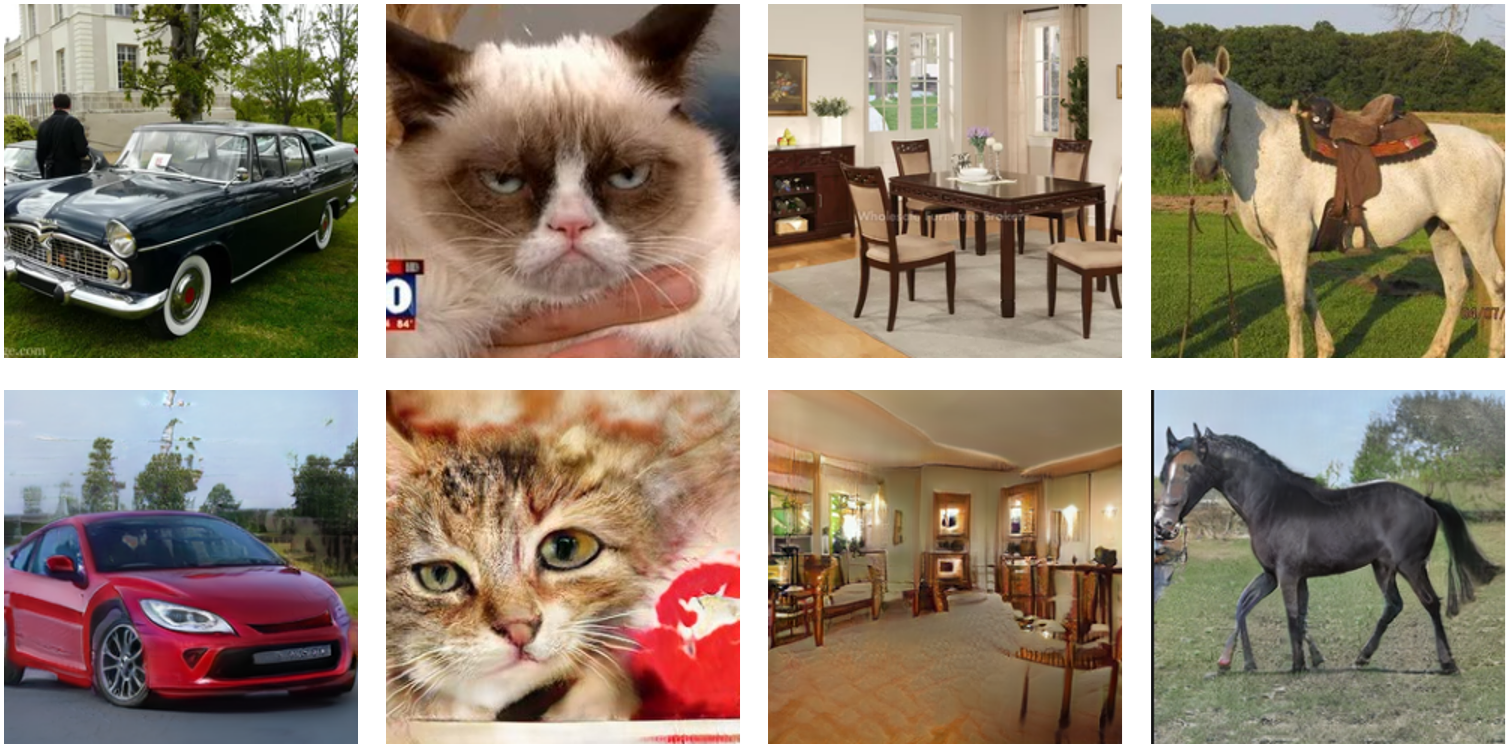
\includegraphics[width=1.0\linewidth]{Images/dataset_progan_samples.png}
	\begin{minipage}{1.0\linewidth}
		\vspace{5mm}
		\caption{Một vài hình ảnh trong tập dữ liệu huấn luyện (các hình ảnh thật ở hàng trên).}
		\label{fig:dataset_progan_samples}
	\end{minipage}
\end{figure}
%

\begin{table}[h]%[htbp]
	\scriptsize 
	\renewcommand{\arraystretch}{1.2} % Tăng chiều cao các hàng lên 1.5 lần
	\centering
	\caption{Tập dữ liệu Forensynths}
	\label{tab:forensynths-dataset}
	\begin{tabular}{|l|c|c|c|c|c|c|}
		\hline
		\textbf{Mô hình} & \textbf{Số lượng} & \textbf{Số danh mục} & \textbf{Tổng cộng} \\ \hline
		ProGAN & 18.000 & 20 & 360.000 \\ 
		StyleGAN  & 18.000 & 20 & 360.000 \\ 
		Stylegan2 & 18.000 & 20 & 360.000 \\  
		BigGAN & 18.000 & 20 & 360.000 \\  
		CycleGAN & 18.000 & 20 & 360.000 \\  
		StarGAN & 18.000 & 20 & 360.000 \\  
		GauGAN & 18.000 & 20 & 360.000 \\  
		Deepfake & 18.000 & 20 & 360.000 \\ 
		\hline
	\end{tabular}
\end{table}

%\vspace{-0.1cm} % Điều chỉnh khoảng cách nếu cần
%\textit{Tất cả hình ảnh trong {Bảng}~\ref{tab:forensynths-dataset} được định dạng (*.png), kích thước} (\( \mathit{256 \times 256 \times 3} \)).


\subsection{Tập dữ liệu dùng cho quá trình đánh giá mô hình}
%
Tập dữ liệu kiểm tra bao gồm các hình ảnh đã được sử dụng trong nhiều công trình nghiên cứu trước đó. Nhằm đánh giá khả năng khái quát của mô hình phát hiện giả mạo,
%
các hình ảnh thật và hình ảnh giả, được sinh từ những mô hình thuộc họ GAN~\cite{Goodfellow2014GenerativeAN} và Diffusion~\cite{Ho2020DenoisingDP}, tương tự như cách tiếp cận trong nghiên cứu của Tan~\cite{Tan2023RethinkingTU}.
%
%
\begin{itemize}
	%\item \textbf{Hình ảnh từ 8 mô hình GAN thuộc bộ dữ liệu ForenSynths}
	%
	\item \textbf{Hình ảnh từ 9 mô hình GAN thuộc bộ dữ liệu Self-Synthesis}~\cite{Tan2023RethinkingTU}, các hình ảnh giả mạo được thu thập từ 9 mô hình GAN~\cite{Goodfellow2014GenerativeAN} khác nhau, bao gồm:
	%
	AttGAN, BEGAN, CramerGAN, InfoMaxGAN, MMDGAN, RelGAN, S3GAN, SNGAN, STGAN. 
	%
	Tổng cộng gồm 36,000 hình ảnh, số lượng hình ảnh thật và giả mạo trong tập dữ liệu là ngang nhau.
	%
	\item \textbf{Hình ảnh từ 8 mô hình Diffusions trong DIRE}~\cite{Wang2023DIREFD}, tác giả sử dụng 8 mô hình Diffusion~\cite{Ho2020DenoisingDP} khác nhau để sinh hình ảnh, bao gồm:
	%
	ADM, DDPM, IDDPM, LDM, PNDM,  Vqdiffusion, Stable Diffusion v1, Stable Diffusion v2.
	%
	Những mô hình này được huấn luyện trên tập ảnh LSUN-Bedroom~\cite{Yu2015LSUNCO} và ImageNet~\cite{5206848}, hình ảnh thật cũng được trích từ hai tập dữ liệu này. Tổng số lượng hình ảnh là 464,000, trong đó 50\% là hình ảnh thật (xem Bảng~\ref{tab:diffusionforensics_dataset}).
	%
	\item \textbf{Hình ảnh từ 4 mô hình Diffusions trong Ojha}~\cite{Ojha2023TowardsUF}, bao gồm 16,000 hình ảnh, trong đó các hình ảnh thật được trích xuất từ tập dữ liệu LAION~\cite{abs-2111-02114}, các hình ảnh giả được tạo từ 4 mô hình Diffusion~\cite{Ho2020DenoisingDP} bao gồm:
	%
	ADM, Glide,  DALL-E-Mini, LDM.
	%
	Quá trình sinh ảnh sử dụng các câu mô tả hình ảnh thật tương ứng để cung cấp thông tin cho mô hình.
	%\item Tập kiểm tra 4
\end{itemize}

\textcolor{red}{Chi tiết của từng tập dữ liệu có thể xem ở phần phụ lục}

\section{Cài đặt huấn luyện và môi trường thực nghiệm}

\subsection{Thiết lập môi trường}

\textbf{Dữ liệu}: Hình ảnh dùng cho huấn luyện thuộc 4 lớp đối tượng \textit{car, cat, chair, horse}, mô hình sinh là ProGAN~\cite{karras2018progressive} thuộc tập Forensynths~\cite{Wang2019CNNGeneratedIA}. Lý do chọn:
\begin{itemize}
	\item Thuận lợi khi so sánh giữa các phương pháp vì đây là tập huấn luyện được nhiều nghiên cứu sử dụng như: Wang~\cite{Wang2019CNNGeneratedIA}, NPR~\cite{Tan2023RethinkingTU}, LGrad~\cite{Tan2023LearningOG}, Ojha~\cite{Ojha2023TowardsUF}. 
	%
	\item Việc chọn hình ảnh giả mạo chỉ từ một mô hình tạo sinh giúp đánh giá tính khái quát và hiệu quả của phương pháp chính xác hơn. Ngoài ra, cách làm này mô phỏng lại tình huống thực tế, khi các mô hình sinh ảnh mới liên tục xuất hiện, trong khi dữ liệu huấn luyện là từ các nguồn cũ và thường cập nhật chậm hơn hoặc không cập nhật.
\end{itemize}

\textbf{Thông số cài đặt:} Được thiết lập tương tự như các phương pháp \cite{Wang2019CNNGeneratedIA, Tan2023RethinkingTU,Tan2023LearningOG} để giảm tác động của các yếu tố ngẫu nhiên đến kết quả cuối cùng, làm mất tính khách quan khi so sánh, đánh giá giữa nhiều phương pháp. Giá trị thiết lập các tham số bao gồm:
	\begin{itemize}
		\item Optimizer: Adam
		\item Learning Rate $2 \times 10^{-4}$
		\item Batch Size: 32
		\item Framework: Các thử nghiệm được xây dựng bằng thư viện PyTorch.
		\item GPU: NVIDIA GeForce RTX 3070 8GB
	\end{itemize}

\subsection{Kết quả quá trình huấn luyện}

\comment{Bảng này cần sửa lại, nên để thông tin quá trình train qua các epoch, và model performance, acc, TPR, FPR...}
\begin{table}[h]%[htbp]
\scriptsize 
\centering
\renewcommand{\arraystretch}{1.2} % Tăng chiều cao các hàng lên 1.5 lần
\caption{Kết quả đánh giá trên tập kiểm tra ForenSynths}
\caption*{\textit{Giá trị thể hiện độ chính xác (accuracy, \%).}}
\label{tab:table1}
\begin{adjustbox}{max width=\textwidth}
\begin{tabular}{|l| cc cc cc cc| c|}
\hline
\multirow{1}{*}{\textbf{Method}} & \multicolumn{1}{c}{\textbf{ProGAN}} & \multicolumn{1}{c}{\textbf{StyleGAN}} & \multicolumn{1}{c}{\textbf{StyleGAN2}} & \multicolumn{1}{c}{\textbf{BigGAN}} & \multicolumn{1}{c}{\textbf{CycleGAN}} & \multicolumn{1}{c}{\textbf{StarGAN}} & \multicolumn{1}{c}{\textbf{GauGAN}} & \multicolumn{1}{c|}{\textbf{Deepfake}} & \multicolumn{1}{c|}{\textbf{Mean}} \\ 
%\cline{2-10}
%& {Acc.} & {Acc.} & {Acc.} & {Acc.} & {Acc.} & {Acc.} & {Acc.} & {Acc.} & {Mean} \\ 
\hline
CNNDetection~\cite{Wang2019CNNGeneratedIA} & 91.4 & 63.8 & 76.4 & 52.9 & 72.7 & 63.8 & 63.9  & 51.7 & 67.1 \\ 
Frank~\cite{Frank2020LeveragingFA} & 90.3 & 74.5 & 73.1 & 88.7 & 75.5 & 99.5 		& 69.2   & 60.7 & 78.9  \\ 
Durall~\cite{Durall2020WatchYU} & 81.1 & 54.4 & 66.8 & 60.1 & 69.0 & 98.1    		& 61.9 & 50.2 & 67.7  \\ 
Patchfor~\cite{Chai2020WhatMF} & 97.8 & 82.6 & 83.6 & 64.7 & 74.5 & 100.0    		& 57.2  & 85.0 & 80.7  \\ 
F3Net~\cite{Qian2020ThinkingIF} & 99.4 & 92.6 & 88.0 & 65.3 & 76.4 & 100.0  		& 58.1  & 63.5 & 80.4 \\ 
SelfBland~\cite{Shiohara2022DetectingDW} & 58.8 & 50.1 & 48.6 & 51.1 & 59.2 & 74.5    & 59.2   & 93.8 & 61.9\\ 
GANDetection~\cite{Mandelli2022DetectingGI} & 82.7 & 74.4 & 69.9 & 76.3 & 85.2 & 68.8 & 61.4   & 60.0 & 72.3  \\ 
BiHPF~\cite{Jeong2021BiHPFBH} & 90.7 & 76.9 & 76.2 & 84.9 & 81.9 & 94.4 			  & 69.5  & 54.4 & 78.6 \\ 
FrePGAN~\cite{Jeong2022FrePGANRD} & 99.0 & 80.7 & 84.1 & 69.2 & 71.1 & 99.9  		  & 60.3  & 70.9 & 79.4 \\ 
LGrad~\cite{Tan2023LearningOG} & 99.9 & 94.8 & 96.0 & 82.9 & 85.3 & 99.6  & 72.4  & 58.0 & 86.1 \\ 
Ojha~\cite{Ojha2023TowardsUF} & 99.7 & 89.0 & 83.9 & 90.5 & 87.9 & 91.4   & 89.9  & 80.2 & 89.1 \\ 
NPR~\cite{Tan2023RethinkingTU} & 99.8 & 96.3 & 97.3 & 87.5 & 95.0 & 99.7  & 86.6  & 77.4 & 92.5 \\ 
{ADOF(our)} & 99.8 & \textbf{99.6} & \textbf{99.5} & 81.1 & 86.1 & 96.8   & 73.4  & 86.0 & 90.3  \\ 
\hline
\end{tabular}
\end{adjustbox}
\end{table}







\section{Đánh giá mô hình}
%
Nội dung đánh giá bao gồm hai phần chính: Thứ nhất, so sánh và đánh giá độ chính xác của nghiên cứu so với các phương pháp tiên tiến hiện nay (Bảng~\ref{tab:table2},\ref{tab:table3},\ref{tab:table4}). Thứ hai, phân tích sâu về hiệu quả sử dụng tài nguyên tính toán và hiệu năng của một số hướng tiếp cận tiêu biểu (xem Bảng ~\ref{tab:model_performance}).
%
%
%
\begin{figure}[ht!]
	\centering
	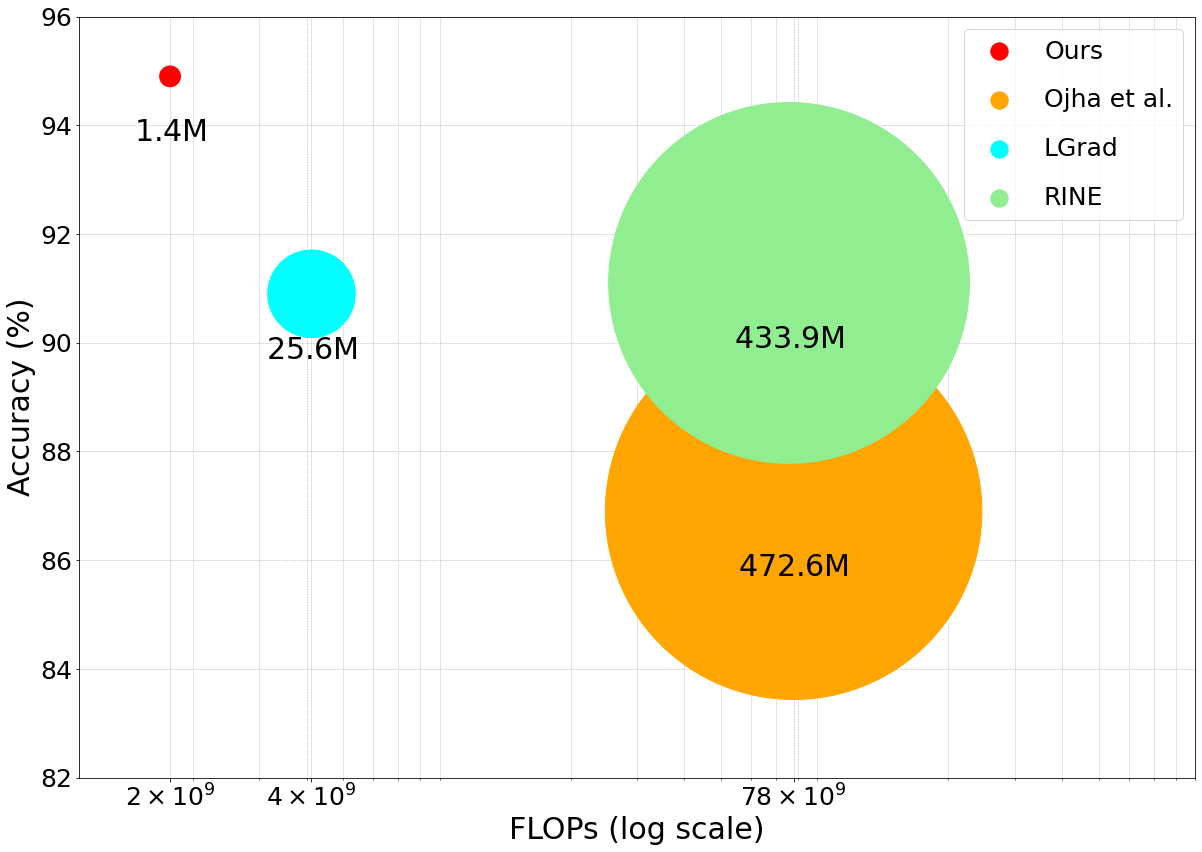
\includegraphics[width=0.7\textwidth]{Images/tease.png}
	%    \fbox{\rule{0pt}{3in} \rule{3in}{0pt}} % Khung ảnh trống
	\caption{Tổng quan hiệu năng và độ chính xác của một số hướng tiếp cận, trên tập dữ liệu Ojha~\cite{Ojha2023TowardsUF}.}
	\label{fig:teaser}
\end{figure}
\subsection{So sánh và đánh giá về độ chính xác}
%\comment{Nhớ thêm chú thích thuật ngữ 'State-of-the-Art'}\\
%
Luận văn thực hiện so sánh độ chính xác của phương pháp đề xuất với 10 phương pháp tiên tiến, bao gồm: 
CNNDetection~\cite{Wang2019CNNGeneratedIA}, 
Frank~\cite{Frank2020LeveragingFA}, 
Durall~\cite{Durall2020WatchYU}, 
Patchfor~\cite{Chai2020WhatMF}, 
F3Net~\cite{Qian2020ThinkingIF}, 
SelfBland~\cite{Shiohara2022DetectingDW}, 
GANDetection~\cite{Mandelli2022DetectingGI}, 
LGrad~\cite{Tan2023LearningOG}, 
Ojha~\cite{Ojha2023TowardsUF}, 
NPR~\cite{Tan2023RethinkingTU}. 
Kết quả thí nghiệm trong các Bảng~\ref{tab:table2}, \ref{tab:table3}, và \ref{tab:table4} cho thấy phương pháp đề xuất vượt trội hơn so với các phương pháp hiện có. 

Trên bộ dữ liệu 9-GAN, ADOF đạt độ chính xác cao nhất là 94.2\%, vượt qua Ojha~\cite{Ojha2023TowardsUF} với chỉ 77.6\% \ref{tab:table2}, và NPR~\cite{Tan2023RethinkingTU} đạt 93.2\% (xem Bảng~\ref{tab:table2}).

Độ chính xác đạt 98.3\% trên tập dữ liệu DiffusionForensics~\cite{Wang2023DIREFD}, cao nhất trong 10 phương pháp, trong khi đó NPR~\cite{Tan2023RethinkingTU} giữ vị trí thứ hai với 95.3\% (xem Bảng~\ref{tab:table3}). Kết quả này cao hơn DIRE~\cite{Wang2023DIREFD} với 97.9\% ngay trên bộ dữ liệu của chính họ, mặc dù mô hình đề xuất trong luận văn được huấn luyện trên Forensynths~\cite{Krizhevsky2012ImageNetCW}, trong khi DIRE được huấn luyện trên DiffusionForensics.

Ngoài ra, độ chính xác cũng trội hơn RINE~\cite{koutlis2024leveraging} và Ojha~\cite{Ojha2023TowardsUF}(91.1\%) (xem Bảng~\ref{tab:table4}). Đáng chú ý, cả hai phương pháp này đều sử dụng mô hình CLIP~\cite{abs-2103-00020} có số lượng tham số rất lớn, yêu cầu nhiều tài nguyên tính toán.

\begin{table}[ht!]%[htbp]
	\centering
	\caption{Kết quả đánh giá trên tập Self-Synthesis 9~GANs~\cite{Tan2023RethinkingTU}.}
	\label{tab:table2}
	\begin{adjustbox}{max width=\textwidth}
		\begin{tabular}{l cc cc cc cc cc cc cc cc cc|cc}
			\toprule
			\vspace{1ex}
			\multirow{2}{*}{{\textbf{Method}}} & \multicolumn{2}{c}{\textbf{AttGAN}} & \multicolumn{2}{c}{\textbf{BEGAN}} & \multicolumn{2}{c}{\textbf{CramerGAN}} & \multicolumn{2}{c}{\textbf{InfoMaxGAN}} & \multicolumn{2}{c}{\textbf{MMDGAN}} & \multicolumn{2}{c}{\textbf{RelGAN}} & \multicolumn{2}{c}{\textbf{S3GAN}} & \multicolumn{2}{c}{\textbf{SNGAN}} & \multicolumn{2}{c|}{\textbf{STGAN}} & \multicolumn{2}{c}{\textbf{Mean}} \\
			\cline{2-21}
			& {\textbf{Acc.}} & {\textbf{A.P.}} & {\textbf{Acc.}} & {\textbf{A.P.}} & {\textbf{Acc.}} & {\textbf{A.P.}} & {\textbf{Acc.}} & {\textbf{A.P.}} & {\textbf{Acc.}} & {\textbf{A.P.}} & {\textbf{Acc.}} & {\textbf{A.P.}} & {\textbf{Acc.}} & {\textbf{A.P.}} & {\textbf{Acc.}} & {\textbf{A.P.}} & {\textbf{Acc.}} & {A.P.} & {\textbf{Acc.}} & {\textbf{A.P.}} \\
			\hline
			CNNDetection~\cite{Wang2019CNNGeneratedIA}  & 51.1 & 83.7 & 50.2 & 44.9 & 81.5 & 97.5 & 71.1 & 94.7  & 72.9 & 94.4 & 53.3 & 82.1 & 55.2 & 66.1 & 62.7 & 90.4 & 63.0 & 92.7 & 62.3 & 82.9 \\
			Frank~\cite{Frank2020LeveragingFA} & 65.0 & 74.4 & 39.4 & 39.9 & 31.0 & 36.0 & 41.1 & 41.0 & 38.4 & 40.5 & 69.2 & 96.2 & 69.7 & 81.9 & 48.4 & 47.9 & 25.4 & 34.0 & 47.5 & 54.7 \\
			Durall~\cite{Durall2020WatchYU} & 39.9 & 38.2 & 48.2 & 30.9 & 60.9 & 67.2 & 50.1 & 51.7 & 59.5 & 65.5 & 80.0 & 88.2 & \textbf{87.3} & 97.0 & 54.8 & 58.9 & 62.1 & 72.5 & 60.3 & 63.3 \\
			Patchfor~\cite{Chai2020WhatMF}  & 68.0 & 92.9 & 97.1 & 100.0 & 97.8 & \textbf{99.9} & 93.6 & 98.2 & 97.9 & \textbf{100.0} & 99.6 & 100.0 & 66.8 & 68.1 & \textbf{97.6} & \textbf{99.8} & 92.7 & 99.8 & 90.1 & 95.4 \\
			F3Net & 85.2 & 94.8 & 87.1 & 97.5 & 89.5 & 99.8 & 67.1 & 83.1 & 73.7 & 99.6 & 98.8 & 100.0 & 65.4 & 70.0 & 51.6 & 93.6 & 60.3 & 99.9 & 75.4 & 93.1 \\
			SelfBland~\cite{Shiohara2022DetectingDW}  & 63.1 & 66.1 & 56.4 & 59.0 & 75.1 & 82.4 & 79.0 & 82.5 & 68.6 & 74.0 & 73.6 & 77.8 & 53.2 & 53.9 & 61.6 & 65.0 & 61.2 & 66.7 & 65.8 & 69.7 \\
			GANDetection~\cite{Mandelli2022DetectingGI} & 57.4 & 75.1 & 67.9 & 100.0 & 67.8 & 99.7 & 67.6 & 92.4 & 67.7 & 99.3 & 60.9 & 86.2 & 69.6 & 83.5 & 66.7 & 90.6 & 69.6 & 97.2 & 66.1 & 91.6 \\
			LGrad~\cite{Tan2023LearningOG}  & 68.6 & 93.8 & 69.9 & 89.2 & 50.3 & 54.0 & 71.1 & 82.0 & 57.5 & 67.3 & 89.1 & 99.1 & 78.5 & 86.0 & 78.0 & 87.4 & 54.8 & 68.0 & 68.6 & 80.8\\
			Ojha~\cite{Ojha2023TowardsUF} & 78.5 & 98.3 & 72.0 & 98.9 & 77.6 & 99.8 & 77.6 & 98.9 & 77.6 & 99.7 & 78.2 & 98.7 & 85.2 & \textbf{98.1} & 77.6 & 98.7 & 74.2 & 97.8 & 77.6 & \textbf{98.8}\\
			NPR~\cite{Tan2023RethinkingTU} &  83.0 & 96.2 & \textbf{99.0} & 99.8 & \textbf{98.7} & 99.0 & \textbf{94.5} & 98.3 & \textbf{98.6} & 99.0 & 99.6 & 100.0 & 79.0 & 80.0 & 88.8 & 97.4 & \textbf{98.0} & \textbf{100.0} & 93.2 & 96.6 \\
			%PatchCraft & 99.7 & 99.99 & 61.1 & 86.0  & 72.4 & 78.4  & 87.5 & 93.3  & 79.8 & 84.3  & 99.5 & 99.9   & 94.0 & 97.9  & 85.1 & 93.2  & 68.6 & 91.3  & 83.1 & 91.6 \\
			\rowcolor{lightgray} {\textbf{ADOF(ours)}} & \textbf{99.5} & \textbf{100.0} & 92.2 & \textbf{100.0} & 96.0 & 99.6 & 94.1 & \textbf{99.1} & 96.0 & 99.7 & \textbf{100.0} & \textbf{100.0} & 77.5 & 86.7 & 94.8 & 99.3 & 97.8 & 99.7 & \textbf{94.2} & 98.2 \\
			\hline
		\end{tabular}
	\end{adjustbox}
\end{table}


\begin{table}[ht!]%[htbp]
	\centering
	\caption{Kết quả đánh giá trên tập DiffusionForensics~\cite{Wang2023DIREFD}.}
	\label{tab:table3}
	\begin{adjustbox}{max width=\textwidth}
		\begin{tabular}{l cc cc cc cc cc cc cc cc|cc}
			\toprule
			%\multirow{2}{*}{\shortstack{Method}} & \multicolumn{2}{c}{\shortstack{ADM}} & \multicolumn{2}{c}{\shortstack{DDPM}} & \multicolumn{2}{c}{\shortstack{IDDPM}} & \multicolumn{2}{c}{\shortstack{LDM}} & \multicolumn{2}{c}{\shortstack{PNDM}} & \multicolumn{2}{c}{\shortstack{VQ-Diffusion}} & \multicolumn{2}{c}{\shortstack{Stable\\Diffusion v1}} & \multicolumn{2}{c}{\shortstack{Stable\\Diffusion v2}} & \multicolumn{2}{c}{\shortstack{Mean}} \\
			\multirow{2}{*}{\shortstack{\textbf{Method}}} & \multicolumn{2}{c}{\shortstack{\textbf{ADM}}} & \multicolumn{2}{c}{\shortstack{\textbf{DDPM}}} & \multicolumn{2}{c}{\shortstack{\textbf{IDDPM}}} & \multicolumn{2}{c}{\shortstack{\textbf{LDM}}} & \multicolumn{2}{c}{\shortstack{\textbf{PNDM}}} & \multicolumn{2}{c}{\shortstack{\textbf{VQ-Diffusion}}} & \multicolumn{2}{c}{\shortstack{\textbf{Stable}\\\textbf{Diffusion v1}}} & \multicolumn{2}{c}{\shortstack{\textbf{Stable}\\\textbf{Diffusion v2}}} & \multicolumn{2}{c}{\shortstack{\textbf{Mean}}} \\
			
			\cline{2-19}
			& \textbf{Acc.} & \textbf{A.P.} & \textbf{Acc.} & \textbf{A.P.} & \textbf{Acc.} & \textbf{A.P.} & \textbf{Acc.} & \textbf{A.P.} & \textbf{Acc.} & \textbf{A.P.} & \textbf{Acc.} & \textbf{A.P.} & \textbf{Acc.} & \textbf{A.P.} & \textbf{Acc.} & \textbf{A.P.} & \textbf{Acc.} & \textbf{A.P.} \\
			
			\hline
			CNNDetection~\cite{Wang2019CNNGeneratedIA}  & 53.9 & 71.8 & 62.7 & 76.6 & 50.2 & 82.7 & 50.4 & 78.7 & 50.8 & 90.3 & 50.0 & 71.0 & 38.0 & 76.7 & 52.0 & 90.3 & 51.0 & 79.8 \\
			Frank~\cite{Frank2020LeveragingFA}  & 58.9 & 65.9 & 37.0 & 27.6 & 51.4 & 65.0 & 51.7 & 48.5 & 44.0 & 38.2 & 51.7 & 66.7 & 32.8 & 52.3 & 40.8 & 37.5 & 46.0 & 50.2 \\
			Durall~\cite{Durall2020WatchYU}  & 39.8 & 42.1 & 52.9 & 49.8 & 55.3 & 56.7 & 43.1 & 39.9 & 44.5 & 47.3 & 38.6 & 38.3 & 39.5 & 56.3 & 62.1 & 55.8 & 47.0 & 48.3 \\
			Patchfor~\cite{Chai2020WhatMF}   & 77.5 & 93.9 & 62.3 & 97.1 & 50.0 & 91.6 & 99.5 & 100.0 & 50.2 & 99.9 & 100.0 & 100.0 & 90.7 & 99.8 & 94.8 & 100.0 & 78.1 & 97.8\\
			F3Net~\cite{Qian2020ThinkingIF} & 80.9 & 96.9 & 84.7 & 99.4 & 74.7 & 98.9 & 100.0 & 100.0 & 72.8 & 99.5 & 100.0 & 100.0 & 73.4 & 97.2 & 99.8 & 100.0 & 85.8 & 99.0 \\
			SelfBland~\cite{Shiohara2022DetectingDW}   & 57.0 & 59.0 & 61.9 & 49.6 & 63.2 & 66.9 & 83.3 & 92.2 & 48.2 & 48.2 & 77.2 & 82.7 & 46.2 & 68.0 & 71.2 & 73.9 & 63.5 & 67.6 \\
			GANDetection~\cite{Mandelli2022DetectingGI}  & 51.1 & 53.1 & 62.3 & 46.4 & 50.2 & 63.0 & 51.6 & 48.1 & 50.6 & 79.0 & 51.1 & 51.2 & 39.8 & 65.6 & 50.1 & 36.9 & 50.8 & 55.4 \\
			LGrad~\cite{Tan2023LearningOG}   & 86.4 & 97.5 & \textbf{99.9} & 100.0 & 66.1 & 92.8 & 99.7 & 100.0 & 69.5 & 98.5 & 96.2 & 100.0 & 90.4 & 99.4 & 97.1 & 100.0 & 88.2 & 98.5 \\
			Ojha~\cite{Ojha2023TowardsUF} & 78.4 & 92.1 & 72.9 & 78.8 & 75.0 & 92.8 & 82.2 & 97.1 & 75.3 & 92.5 & 83.5 & 97.7 & 56.4 & 90.4 & 71.5 & 92.4 & 74.4 & 91.7\\
			NPR~\cite{Tan2023RethinkingTU}  & 88.6 & 98.9 & 99.8 & 100.0 & 91.8 & 99.8 & 100.0 & 100.0 & 91.2 & \textbf{100.0} & 100.0 & 100.0 & 97.4 & 99.8 & 93.8 & 100.0 & 95.3 & 99.8 \\
			\rowcolor{lightgray} {\textbf{ADOF(ours)}} & \textbf{93.5} & \textbf{99.0} & 99.6 & \textbf{100.0} & \textbf{99.2} & \textbf{100.0} & 99.9 & \textbf{100.0} & \textbf{97.4} & 99.9 & 97.1 & 99.8 & \textbf{99.8} & \textbf{100.0} & \textbf{99.9} & \textbf{100.0} & \textbf{98.3} & \textbf{99.8} \\
			
			\bottomrule
		\end{tabular}
	\end{adjustbox}
\end{table}




\begin{table}[ht!]%[htbp]
	\caption{Kết quả đánh giá trên tập Ojha~\cite{Ojha2023TowardsUF}.}
	\label{tab:table4}
	\centering
	\begin{adjustbox}{max width=\textwidth}
		\begin{tabular}{l cc cc cc cc cc cc cc cc|cc}
			\hline
			\multirow{2}{*}{{\textbf{Method}}} & \multicolumn{2}{c}{\textbf{DALLE}} & \multicolumn{2}{c}{$\mathbf{{Glide_{(100\_10)}}}$} & \multicolumn{2}{c}{$\mathbf{{Glide_{(100\_27)}}}$} & \multicolumn{2}{c}{$\mathbf{{Glide_{(50\_27)}}}$} & \multicolumn{2}{c}{\textbf{ADM}} & \multicolumn{2}{c}{$\mathbf{{LDM_{(100)}}}$} & \multicolumn{2}{c}{$\mathbf{{LDM_{(200)}}}$} & \multicolumn{2}{c|}{$\mathbf{{LDM_{(200\_cfg)}}}$} & \multicolumn{2}{c}{\textbf{Mean}} \\
			\cline{2-19}
			& {\textbf{Acc.}} & {\textbf{A.P.}} & {\textbf{Acc.}} & {\textbf{A.P.}} & {\textbf{Acc.}} & {\textbf{A.P.}} & {\textbf{Acc.}} & {\textbf{A.P.}} & {\textbf{Acc.}} & {\textbf{A.P.}} & {\textbf{Acc.}} & {\textbf{A.P.}} & {\textbf{Acc.}} & {\textbf{A.P.}} & {\textbf{Acc.}} & {\textbf{A.P.}} & {\textbf{Acc.}} & {\textbf{A.P.}} \\
			
			\hline
			CNNDetection~\cite{Wang2019CNNGeneratedIA}  & 51.8 & 61.3 & 53.3 & 72.9 & 53.0 & 71.3 & 54.2 & 76.0 & 54.9 & 66.6 & 51.9 & 63.7 & 52.0 & 64.5 & 51.6 & 63.1 & 52.8 & 67.4 \\
			Frank~\cite{Frank2020LeveragingFA}   & 57.0 & 62.5 & 53.6 & 44.3 & 50.4 & 40.8 & 52.0 & 42.3 & 53.4 & 52.5 & 56.6 & 51.3 & 56.4 & 50.9 & 56.5 & 52.1 & 54.5 & 49.6 \\
			Durall~\cite{Durall2020WatchYU}  & 55.9 & 58.0 & 54.9 & 52.3 & 48.9 & 46.9 & 51.7 & 49.9 & 40.6 & 42.3 & 62.0 & 62.6 & 61.7 & 61.7 & 58.4 & 58.5 & 54.3 & 54.0 \\
			Patchfor~\cite{Chai2020WhatMF}   & 79.8 & {99.1} & 87.3 & 99.7 & 82.8 & 99.1 & 84.9 & 98.8 & 74.2 & 81.4 & 95.8 & 99.8 & 95.6 & 99.9 & 94.0 & 99.8 & 86.8 & 97.2 \\
			F3Net~\cite{Qian2020ThinkingIF}  & 71.6 & 79.9 & 88.3 & 95.4 & 87.0 & 94.5 & 88.5 & 95.4 & 69.2 & 70.8 & 74.1 & 84.0 & 73.4 & 83.3 & 80.7 & 89.1 & 79.1 & 86.5 \\
			SelfBland~\cite{Shiohara2022DetectingDW}    & 52.4 & 51.6 & 58.8 & 63.2 & 59.4 & 64.1 & 64.2 & 68.3 & 58.3 & 63.4 & 53.0 & 54.0 & 52.6 & 51.9 & 51.9 & 52.6 & 56.3 & 58.7 \\
			GANDetection~\cite{Mandelli2022DetectingGI}  & 67.2 & 83.0 & 51.2 & 52.6 & 51.1 & 51.9 & 51.7 & 53.5 & 49.6 & 49.0 & 54.7 & 65.8 & 54.9 & 65.9 & 53.8 & 58.9 & 54.3 & 60.1 \\
			LGrad~\cite{Tan2023LearningOG}    & 88.5 & 97.3 & 89.4 & 94.9 & 87.4 & 93.2 & 90.7 & 95.1 & \textbf{86.6} & \textbf{100.0} & 94.8 & 99.2 & 94.2 & 99.1 & 95.9 & 99.2 & 90.9 & 97.2 \\
			Ojha~\cite{Ojha2023TowardsUF}   & 89.5 & 96.8 & 90.1 & 97.0 & 90.7 & 97.2 & 91.1 & 97.4 & 75.7 & 85.1 & 90.5 & 97.0 & 90.2 & 97.1 & 77.3 & 88.6 & 86.9 & 94.5 \\
			NPR~\cite{Tan2023RethinkingTU}   & {94.5} & \textbf{99.5} & 98.2 & 99.8 & 97.8 & 99.7 & 98.2 & 99.8 & 75.8 & 81.0 & \textbf{99.3} & 99.9 & \textbf{99.1} & 99.9 & \textbf{99.0} & 99.8 & \textbf{95.2} & 97.4 \\
			%PatchCraft & 83.3 & 93.0 & 80.1 & 92.0  & 83.4 & 93.9  & 77.6 & 88.7 & 80.9 & 90.5  & 88.9 & 97.7  & 89.3 & 97.9  & 88.1 & 96.9 & 84.0 & 93.8 \\
			RINE~\cite{koutlis2024leveraging}   & \textbf{95.0} & 99.5 & 90.7 & 99.2 & 88.9 & 99.1 & 92.6 & 99.5 & 76.1 & 96.6 & {98.7} & 99.9 & {98.3} & 99.9 & 88.2 & 98.7 & {91.1} & 99.0 \\
			\rowcolor{lightgray}{\textbf{ADOF(ours)}} & 92.1 & 98.3 & \textbf{98.6} & \textbf{100.0} & \textbf{98.7} & \textbf{100.0} & \textbf{98.4} & \textbf{99.9} & 75.9 & 87.6 & 98.8 & \textbf{100.0} & 98.6 & \textbf{99.9} & 98.5 & \textbf{99.9} & 94.9 & \textbf{98.2} \\
			
			\hline
		\end{tabular}
	\end{adjustbox}
\end{table}

%RINE Ojha 4-class
%dalle: 95.0 / 99.5
%glide_100_10: 90.7 / 99.2
%glide_100_27: 88.9 / 99.1
%glide_50_27: 92.6 / 99.5
%guided: 76.1 / 96.6
%ldm_100: 98.7 / 99.9
%ldm_200: 98.3 / 99.9
%ldm_200_cfg: 88.2 / 98.7
%Mean: 91.1 / 99.0
\subsection{So sánh và đánh giá về hiệu năng}
%
%
Để so sánh về hiệu năng, luận văn thực hiện đo lường các tiêu chí về độ phức tạp của mô hình cũng như số lượng phép toán cần thiết cho mỗi dự đoán (chi tiết xem Bảng~\ref{tab:model_performance}). Tất cả được thực hiện trên máy tính có CPU AMD Ryzen 5 5600X 6-Core, GPU NVIDIA RTX A4000, 16 GB bộ nhớ RAM. Hình ảnh đầu vào có kích thước $256 \times 256 \times 3$. Các tiêu chí đánh giá bao gồm:
%
\begin{figure}[ht!]
	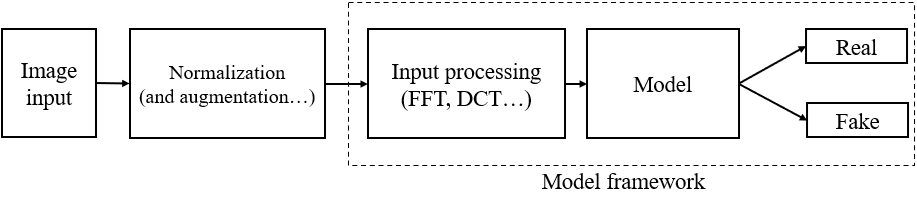
\includegraphics[width=\textwidth]{Images/figure_pine_line_1.png}
	\caption{Quy trình cơ bản của mô hình phát hiện ảnh tạo sinh}	
	\label{figure_pine_line_1}
\end{figure}
%
%
\begin{itemize}
	\item \textbf{Number of Parameters:} Số lượng tham số của mô hình, thể hiện độ phức tạp trong kiến trúc.
	\item \textbf{Input Processing Time:} Đo lường thời gian cần thiết để xử lý hình ảnh trước khi đưa vào mô hình dự đoán, các bước xử lý này thay đổi theo hướng tiếp cận cụ thể (xem Hình.~\ref{figure_pine_line_1}).
	\item \textbf{Inference Time:} Thời gian cần sử dụng cho một dự đoán.
	\item \textbf{FLOPs:} Số lượng phép tính dấu chấm động trong 1 giây, luận văn sử dụng thư viện \texttt{fvcore} để ước tính khối lượng tính toán mà mỗi mô hình cần thực hiện cho một dự đoán.
\end{itemize}
%
%
\begin{table}[h!]
	\centering
	\caption{Tài nguyên sử dụng và hiệu năng của các phương pháp phát hiện hình ảnh tổng hợp, trên tập dữ liệu DiffusionForensics~\cite{Wang2023DIREFD}. Dấu \textsuperscript{$\dagger$} thể hiện phương pháp đã được huấn luyện trên cùng tập dữ liệu.}
	\label{tab:model_performance}
	\begin{adjustbox}{max width=\textwidth}
		\setlength{\tabcolsep}{12pt} % Tăng khoảng cách giữa các cột cho bảng này
		\renewcommand{\arraystretch}{1.1} % Điều chỉnh chỉ cho bảng này
		\begin{tabular}{l c c c c c}
			\toprule
			\multirow{2}{*}{\textbf{Method}} &
			\multirow{2}{*}{\textbf{Parameters}} &
			\multirow{2}{*}{\begin{tabular}[c]{@{}c@{}}\textbf{Processing} \\ \textbf{(ms)}\end{tabular}} &
			\multirow{2}{*}{\begin{tabular}[c]{@{}c@{}}\textbf{Inference Time}\\ \textbf{(ms)}\end{tabular}} &
			\multirow{2}{*}{\textbf{FLOPs}} &
			\multirow{2}{*}{\begin{tabular}[c]{@{}c@{}}\textbf{Means} \\ \textbf{(acc/ap)} \end{tabular}} \\
			&   &   &   &   &    \\ \hline
			LGrad~\cite{Tan2023LearningOG} (2023) & {$25.56 \times 10^6$} & {11.6} & {4.81} & {$4.12 \times 10^9$} & {88.2/98.5}\\ %\hline
			%LNP & {$23.51 \times 10^6$} & {65.6} & -- & {$4.12 \times 10^9$} & {--}\\ %\hline
			DIRE\textsuperscript{$\dagger$}~\cite{Wang2023DIREFD} (2023) & {$25.56 \times 10^6$} & {4,502.7} & {4.81} & {$4.12 \times 10^9$} & {97.9/\textbf{100}}\\ %\hline
			Ojha~\cite{Ojha2023TowardsUF} (2023) & {$427.62 \times 10^6$} & {None} & {29.19} & {$77.83 \times 10^9$} & {74.4/91.7}\\ %\hline
			%PatchCraft~\cite{zhong2024patchcraftexploringtexturepatch} & {$\mathbf{0.12 \times 10^6}$} & {--} & {--} & {$6.70 \times 10^9$} & {84.0/92.7}\\ %\hline
			\rowcolor{lightgray} \textbf{ADOF(ours)} & {\textbf{$1.44 \times 10^6$}} & 0.40 & \textbf{2.43} & {$\mathbf{1.74 \times 10^9}$} & {\textbf{98.3}/99.8}\\ \bottomrule
		\end{tabular}
	\end{adjustbox}
\end{table}






